% This version uses the latex2e styles, not the very ancient 2.09 stuff.
\documentclass{sig-alternate-10pt}
\usepackage{endnotes,url}
%\usepackage{sig-alternate-10pt,endnotes}
\usepackage{epsfig}
\usepackage{amssymb}
\usepackage{amsmath}
\usepackage{lipsum}
\usepackage{algorithm}
\usepackage{algorithmic}
\usepackage{amsfonts}
\usepackage{graphicx}
\usepackage{verbatim}
% Replaced by subfig package
% \usepackage{subfigure}
\usepackage{subfig}
\usepackage{epstopdf}
\usepackage{cite}
\usepackage{array}
\usepackage{multirow}
\usepackage{listings}

\captionsetup[figure]{labelfont={small},textfont={small}}

%\pdfpagewidth 8.5in
%\pdfpageheight 11in
%\baselineskip=12.5pt
%\setlength{\pdfpagewidth}{8.5in}
%\setlength{\pdfpageheight}{11in}
%\usepackage{pdfdraftcopy}

% To import classical math notation used

% Mathematical LaTeX formatting shortcuts
\newcommand{\midwor}[1]{\;\textnormal{ #1 }\;} % text in math mode
\newcommand{\ds}{\displaystyle} % shorcut to toggle display
	% All formula should punctuation as they are part of the text.
\newcommand{\vf}{\,,\,} % a comma with space
\newcommand{\ff}{\,.} % a dot 
	% The following command allows to write quickly sets { }   
\newcommand{\lset}{\left\{\left.\;}
\newcommand{\midset}{\;\right|\;\left.}
\newcommand{\dimset}{\right.\;\left|\;}
\newcommand{\rset}{\;\right.\right\}}
\newcommand{\jset}{\right.\right.\\ & \left.\left.}

% Number sets and usual operations
\newcommand{\Real}{\mathbb{R}} % real numbers
\newcommand{\RelInt}{\mathbb{Z}} % relative integer numbers
\newcommand{\NatInt}{\mathbb{N}} % natural integer numbers
\newcommand{\Compl}{\mathbb{C}} % complex numbers
\newcommand{\valent}[1]{\left\lfloor #1 \right\rfloor} % integer value
\newcommand{\valentsup}[1]{\left\lceil #1 \right\rceil} % integer value + 1
\newcommand{\eps}{\varepsilon} % very small real number
\newcommand{\argmin}{\textrm{argmin}} %argument of the minimum
\newcommand{\pospar}[1]{\left( #1 \right)^+} % positive part

% Probability notation
\newcommand{\proba}{\mathbb{P}} % Probability
\newcommand{\probaof}[1]{\mathbb{P}\left.\left[#1\right.\right]} % Probability of an event
\newcommand{\cond}{\right|\left.} % Condition on an event 
\newcommand{\expec}[1]{\mathbb{E}\left[#1\right]} % Expectation 
\newcommand{\vari}[1]{\textrm{V}\left[#1\right]} % Variance 
\newcommand{\Lun}{\mathbb{L}^{1}} % Space of integrable function
\newcommand{\as}{\;\textrm{a.s.}\;}
\newcommand{\ind}[1]{\mathbb{I}_{\{#1\}}} % Indicator
\newcommand{\tribF}{\mathcal{F}} % sigma-algebra

% Constants
\newcommand{\cst}{\textrm{\texttt{cst}}}

% Advanced probability 
\newcommand{\comp}{\circ} % composition of function
\newcommand{\shi}{\theta} % ergodic shift
\newcommand{\lstoc}{\displaystyle \leq_{\textrm{st}}} % Stochastic Order
\newcommand{\Ppalmof}[1]{\mathbb{P}^{0}_{#1}}
\newcommand{\Pofpalmof}[2]{\mathbb{P}^{0}_{#1}\left[#2\right]}
\newcommand{\expPalm}[1]{\mathbb{E}^{0}[#1]} % Palm Expectation
\newcommand{\expPalmof}[2]{\mathbb{E}^{0}_{#1}[#2]} % Palm Expectation w.r.t. point process f 

% (max,+) algebra
\newcommand{\Rmax}{\mathbb{R}_{\max}}
\newcommand{\ninf}{\varepsilon}
\newcommand{\matninf}{\textrm{\Large{$\ninf$}}}
\newcommand{\zer}{e}
\newcommand{\veczer}{\textrm{\Large{e}}}
\newcommand{\bigmax}{\bigvee}
\newcommand{\matId}{{\mathbb{I}}}
%\newcommand{\norm}[1]{\| #1 \|}
\newcommand{\linf}[1]{\left|\left| #1 \right|\right|}

% Matrices
\newcommand{\matA}{\mathbb{A}}
\newcommand{\matB}{\mathbb{B}}
\newcommand{\matC}{\mathbb{C}}
\newcommand{\matP}{\mathbb{P}}
\newcommand{\matQ}{\mathbb{Q}}

% Used for set
\newcommand{\setI}{\mathcal{I}}
\newcommand{\setJ}{\mathcal{J}}
\newcommand{\setK}{\mathcal{K}}
\newcommand{\setL}{\mathcal{L}}

% Users and Buckets
\newcommand{\setU}{\mathcal{U}}
\newcommand{\setC}{\mathcal{C}}

\newcommand{\setA}{\mathcal{A}}
\newcommand{\setW}{\mathcal{W}}

% Used for set
\newcommand{\setN}{\mathcal{N}}
\newcommand{\setS}{\mathcal{S}}


\newenvironment{disarray}%
 {\everymath{\displaystyle\everymath{}}\array}%
 {\endarray}

 \newcommand{\pdi}[1]{\frac{\partial #1}{\partial x_i}}
 \newcommand{\pdj}[1]{\frac{\partial #1}{\partial x_j}}

% Package for date and time presentation
\usepackage{datetime}
\newcommand{\datation}{\today, \xxivtime}

\def\full{0}        % set 1 for a full tech report version
                    % set 0 for submission version
\def\shownotes{1}   % set 1 for version with author notes
                    % set 0 for no notes
\def\anon{1}        % set 1 to anonymize
                    % set 0 for acks and author names

%%%%%%%  Author Notes %%%%%%%
%
\ifnum\shownotes=1
\newcommand{\authnote}[2]{{ $\ll$\textsf{\footnotesize #1 notes: #2}$\gg$}}
\else
\newcommand{\authnote}[2]{}
\fi
\newcommand{\Anote}[1]{{\authnote{Andrius}{#1}}}

%%%%%%%%%%%%%%%%%%%%%%%%%%%%%%%%%

\newcommand{\namedref}[2]{#1~\ref{#2}}
\newcommand{\tableref}[1]{\namedref{Table}{#1}}
\newcommand{\sectionref}[1]{\namedref{Section}{#1}}
\newcommand{\appendixref}[1]{\namedref{Appendix}{#1}}
\newcommand{\theoremref}[1]{\namedref{Theorem}{#1}}
\newcommand{\remarkref}[1]{\namedref{Remark}{#1}}
\newcommand{\definitionref}[1]{\namedref{Definition}{#1}}
\newcommand{\figureref}[1]{\namedref{Figure}{#1}}
\newcommand{\lemmaref}[1]{\namedref{Lemma}{#1}}
\newcommand{\claimref}[1]{\namedref{Claim}{#1}}
\newcommand{\propositionref}[1]{\namedref{Proposition}{#1}}
\newcommand{\constructionref}[1]{\namedref{Construction}{#1}}
\newcommand{\corollaryref}[1]{\namedref{Corollary}{#1}}
\newcommand{\equationref}[1]{\namedref{Equation}{#1}}
%
\newtheorem{theorem}{Theorem}[section]
\newtheorem{definition}[theorem]{Definition}
\newtheorem{lemma}[theorem]{Lemma}
\newtheorem{claim}[theorem]{Claim}
\newtheorem{obs}[theorem]{Observation}
%


\providecommand{\vs}{vs. }
\providecommand{\ie}{\emph{i.e.,} }
\providecommand{\eg}{\emph{e.g.,} }
\providecommand{\cf}{\emph{cf.,} }
\providecommand{\resp}{\emph{resp.,} }
\providecommand{\etal}{\emph{et al.}}   %Removed trailing space here; usually want non-breaking space with following reference
\providecommand{\etc}{\emph{etc.}}      % No trailing space here either
\providecommand{\mypara}[1]{\smallskip\noindent\emph{#1} }
\providecommand{\myparab}[1]{\smallskip\noindent\textbf{#1} }
\providecommand{\myparasc}[1]{\smallskip\noindent\textsc{#1} }
\providecommand{\para}{\smallskip\noindent}

\newtheorem{axiom}{{\bf  Axiom}}
\newtheorem{defin}{{\bf  Definition}}
\newtheorem{proposition}{Proposition}

\usepackage{enumitem}
\setlist{nolistsep}

%Model parameters

\usepackage[breaklinks=true]{hyperref}
\frenchspacing

\setlength{\paperheight}{11in}
\setlength{\paperwidth}{8.5in}
\usepackage[
  pass,% keep layout unchanged 
  % showframe,% show the layout
]{geometry}

\begin{document}

%don't want date printed
\date{}


%make title bold and 14 pt font (Latex default is non-bold, 16 pt)
\title{NoTCP: steganographic tricks to bypass middleboxes}
\ifnum\anon=1
\author{[Paper: \#137]}% \hspace{0.2cm} \ampmtime ]}
\else
\numberofauthors{3}
\author{
\alignauthor Andrius Aucinas\\
\affaddr{University of Cambridge} 
\and
\alignauthor Jon Crowcroft\\
\affaddr{University of Cambridge}
\and
\alignauthor Narseo Vallina-Rodriguez\\
\affaddr{ICSI}
}
\fi
%for single author (just remove % characters)

    
% end author
\maketitle
% Use the following at camera-ready time to suppress page numbers.
% Comment it out when you first submit the paper for review.
%\thispagestyle{empty}
\begin{abstract}
TCP is the de facto transport protocol in the Internet. However it has many limitations that make it ill-suited to the modern world of high mobility and multi-homing. Protocol optimizations and filtering performed by middleboxes make extension deployment challenging. This has led researchers to explore new ways of exchanging control information between endpoints. We present NoTCP -- a mechanism which uses the TCP header fields in combinations that have no defined semantics in order to hide a small amount of control information from middleboxes and hence bootstrap a control channel. We also present a preliminary study showing how the mechanism works across cellular and WiFi networks.
\end{abstract} 

\section{Introduction}
\label{section:intro}

Over the last decade a number of new protocols have been proposed to replace TCP. However many middleboxes will actively block or interfere with traffic that does not conform to their view of what TCP should look like~\cite{Handley:2001vp,Vutukuru:2008fc,Guha2005tb}. Consequently, few of these protocols have seen real deployment.

One of the main requirements to extend and modify TCP is the ability to exchange control information. Traditionally this is what TCP option space was used for. However option space is limited, heavily contended~\cite{Handley:vj,Mazieres:uz} and network middleboxes make it difficult to use because of inconsistent interpretation of the specifications~\cite{Honda,Guha2005tb,UntoldMiddlebox2011}. On the other hand, modern networks demand new protocols for mobile and multi-homed devices~\cite{Mazieres:uz}, ubiquitous traffic encryption~\cite{Handley:vj,Rescorla:R080FoGB}, energy efficiency~\cite{Aucinas:2013uk}, connection parameters tuning for specific workloads and environments~\cite{Dukkipati:2010hs,Erman:2013uz} that were unknown 30 years ago.

One solution is to work round the middleboxes by using steganographic techniques~\cite{Frczek:2012dl,Zielinska:2014fn,Rowland:1997vq,Murdoch:2005fz} to conceal control information within the TCP header beyond the sight of middleboxes. This could be as simple as using one of the currently undefined flags to toggle the meaning of existing fields, through to using the urgent pointer without setting the urgent flag or even hashing information into the initial sequence number in much the way that TCP Fast Open~\cite{Chu:2011tn} does for application data delivery.

Steganographic communication channels are typically low bandwidth and statistical analysis of a sufficient amount of data usually exposes the existence of such channels~\cite{Murdoch:2005fz}. Nevertheless, it is the perfect choice for exchanging a small amount of end-to-end control data in real-time and it does not compromise network security since the channel can be detected using existing techniques. In our work we discuss the possible ways to conceal information in the TCP header and present the results of a preliminary study on the suitability of various header fields for the purpose.

We use our initial study to design a way of exchanging a small amount of control information successfully across all of our tested networks and show a potential mechanism to use it for bootstrapping a full control stream currently missing from TCP.

Our approach is not a short-term hack. Many recent proposals have demonstrated that control over end-to-end protocol behavior should remain at the endpoints. These include TCPCrypt which offers improved communication confidentiality and security and TCP Fast Open for better communication performance. We hope that our successful results will motivate the research community into exploring the full range of possibilities in this space.

\section{Candidate protocol changes}
\label{sec:protocolChanges}

\begin{figure}[t!]
\centering
\small{
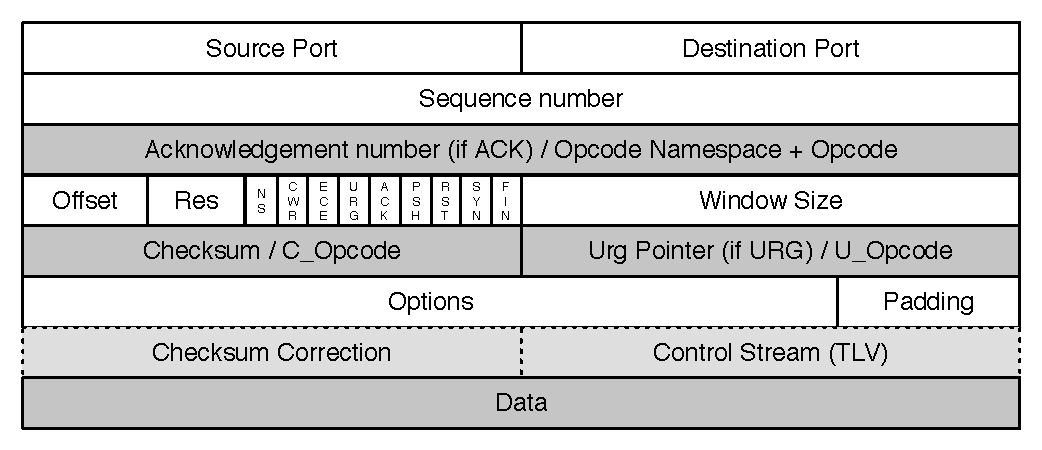
\includegraphics[width=\columnwidth]{figs/tcp-header}
% \vspace{-5mm}
\caption{TCP Header with overloaded fields and extra control information (Checksum Correction / Control Stream) in payload. Fields in gray used for control information. Light-gray fields are optional and are within payload.}
\label{fig:header}
}
\vspace{-4mm}
\end{figure}

Design of a control channel is constrained by protocol specification and its interpretation by middleboxes. In the past, TCP sequence numbers~\cite{Murdoch:2005fz}, timestamps~\cite{Giffin:2002wh} and IP ID~\cite{Ahsan:2002wc} have been used for encoding hidden information. In our work we focus on a different set of TCP header fields (Fig.~\ref{fig:header}, in gray, defined in \S\ref{sec:protocol}). Overall, the header leaves few options for hiding control information:
\begin{itemize}
    \item Setting fields without the corresponding flags so they have no meaning to legacy implementations.
    \item Assigning one or more of the reserved field bits.
    \item Overloading the semantics for valid header fields.
\end{itemize}

\subsubsection*{Flag-dependent semantics}
\label{sec:unset}

Only two header fields have their semantics set by corresponding flags. These are the \emph{Acknowledgment Number} (which must always be set after the initial SYN packet) and the \emph{Urgent Pointer}. 

The Acknowledgment Number field is only available in the initial SYN packet, but is usable across our tested networks (\S\ref{sec:network}). It must therefore be combined with another mechanism to acknowledge control information unless TCP Simultaneous Open is used. Simultaneous open is still viable in most cellular networks~\cite{UntoldMiddlebox2011}, but we also explore other options.

The general recommendation is to not use the urgent mechanism~\cite{Gont:2011vi}. The \emph{Urgent Pointer} could therefore be reused for other purposes as long as both endpoints understand the new semantics and middleboxes permit it. On the other hand, Network Intrusion Detection Systems (NIDS) often reset the field as it makes it difficult to track application-layer data~\cite{seolma}. Importantly, the field becomes \emph{Non-Urgent}~\cite{Kuhlewind:2014vd} when URG is not set -- it has no meaning for legacy implementations and so can be redefined if middleboxes permit it as they often do (\S\ref{sec:network}).

\subsubsection*{Reserved bits}
\label{sec:reserved}

Three TCP reserved bits remain unallocated. One further bit is only allocated to the experimental ECN nonce\cite{Ely:uc}. Despite their limited size, there are proposals that make use of new reserved bits due to implementation simplicity and non-interference with legacy implementations. One suggestion for reducing Web latency~\cite{Flach:2013uy} by mitigating the effects of a small number of lost packets for short connections is to send multiple copies of packets. The proposal deliberately sends copies, but uses a reserved flag to explicitly mark solution avoids triggering fast retransmit by such duplicate acknowledgments by marking them as duplicates in a reserved flag.

\subsubsection*{Value-specific semantics}

The remaining choice is to encode information within otherwise valid header fields. It involves generating packets with specific values for \emph{Initial Sequence Numbers}, \emph{Window Size} or \emph{Checksums}. Arguably it is an acceptable choice if deployable in today's networks. Indeed SYN Cookies already do this~\cite{Eddy:2007to}

\emph{Initial Sequence Numbers} must be hard to predict as they provide a measure of security against TCP injection attacks. Adding information to the field to be easily decoded by the receiver makes it more predictable and weakens already problematic security~\cite{Bellovin:uz,Qian:2012wb}. Also some stateful middleboxes are known to interfere with sequence numbers in an attempt to improve security~\cite{Qian:2012bj}. Stronger security measures such as TCPCrypt~\cite{Mazieres:uz} are better suited for connection protection.

\emph{Window Size} is potentially a better candidate, especially if used during connection setup phase since data is not typically transmitted during the handshake. Using lower-order bits for control information would prevent flow control from operating properly, but higher-order bits could instead be given up when the \emph{window scaling} option is used to compensate for the decrease of advertised window size. Using the field risks interfering both with TCP flow control mechanism as well as window size optimizations by the network~\cite{Kopparty:2002ht,Chakravorty:2003dm} performed by \eg Citrix ByteMobile Proxy~\cite{Ha:2006td}. 

There are multiple benefits to using the checksum field. Firstly, it is only used for error detection. It may be unnecessary when reliable error detection is done at the layer below, however link-level checks have been shown to be unreliable~\cite{Stone:2000fc}. Instead, it may be replaced with potentially stronger mechanisms such as MPTCP DSS checksum and TCPCrypt Message Authentication Code or left for the upper layer. Secondly, checksum operations are efficient as they only involve one's complement addition. We show later in the paper (\S\ref{sec:protocol}) how checksums can be generated in a way that the intended value is recovered by the receiver after traversing multiple layers of Network Address Translation (NAT).

\section{Measurement Methodology}

To measure current network behavior we have developed an Android application distributed through the \emph{Google Play Store}\footnote{Link omitted to anonymize submission} to collect data from volunteers. It contains a simplified implementation of TCP which generates packet sequences that appear valid to network middleboxes: three-way handshake, data exchange and connection teardown. It allows us to modify various header fields and check the values received by the other endpoint. We control both endpoints of each connection, therefore we can detect changes from sent values received by the other endpoint.

The test setup is:
\begin{itemize}
    \item Android application with a simplified TCP stack using Raw Unix sockets for full control over the TCP header (\emph{SOCK\_RAW}). It manages the tests and sends results back to our servers. 
    \item Server instrumented to generate specific responses to incoming packets based on header and payload values. We currently use a dedicated test server in a single location and no firewalls or NATs.
\end{itemize}

Non-transparent proxies are a major problem for extension deployment, therefore we used another well know and widely deployed tool to detect proxies on our tested networks. We implemented previously developed techniques~\cite{Weaver:RHwbx82O} and run the test separately. The primary one was non-responsive server test: the server is instrumented not to respond to SYN, therefore if the connection succeeds it is to a proxy on the path. We repeated these tests on different destination ports and found that proxying can be specific to certain port numbers.

Our methodology avoids packet splitting by only using small packets. Coalescing is prevented by only exchanging a single data message each way. For the same reason we do not take congestion control into account.

\emph{Raw sockets} operate in parallel to the kernel network stack. We had to suppress reset packets generated by the kernel in response to TCP packets from sessions it is not aware of. We also had to choose local port numbers unused by the kernel. We chose them randomly from the unprivileged port range and relied on other error detection mechanisms preventing invalid packet delivery to any applications.

\section{Preliminary Results}
\label{sec:network}

\begin{table*}[t]
{\small
\begin{center}
\begin{tabular}{| l | >{\centering\arraybackslash}m{1.3cm} | >{\centering\arraybackslash}m{1.6cm} | >{\centering\arraybackslash}m{2.4cm} | >{\centering\arraybackslash}m{2.4cm} | >{\centering\arraybackslash}m{2.3cm} | >{\centering\arraybackslash}m{1.5cm} | >{\centering\arraybackslash}m{1.5cm} | >{\centering\arraybackslash}m{1.cm} | }
\hline
    \textbf{Net ID} & \textbf{Port-specific} & \textbf{Validate checksum} & \textbf{Drop SYN-ACK data} & \textbf{Normalize SYN Ack number}  & \textbf{Normalize Urgent Pointer} & \textbf{Normalize Reserved} & \textbf{Remap Sequence} \\ \hline \hline
    % Univ Helsinki WiFi
    WiFi edu 1      &                        & \checkmark                 &                        &                         &                        &                             &                     \\ \hline
    % Eduroam
    WiFi edu 2      &                        &                            & \checkmark             &                         & \checkmark             &                             & \checkmark          \\ \hline
    % wgb
    WiFi pub 1      &                        &                            &                        &                         &                        &                             &                     \\ \hline
    % MKSW germany (carlos)
    WiFi pub 2      &                        & \checkmark                 & \checkmark             &                         &                        &                             &                     \\ \hline
    % Virgin home
    WiFi res 1      &                        & \checkmark                 &                        &                         &                        &                             &                     \\ \hline
    % TEO Lt
    WiFi res 2      &                        & \checkmark                 & \checkmark             &                         &                        &                             &                     \\ \hline
    % Telefonica Free
    WiFi ent 1      &                        & \checkmark                 & \checkmark             &                         &                        &                             &                     \\ \hline
    \hline
    % Finland internet.saunalahti
    Cellular 1      &                        &                            &                        &                         &                        &                             &                     \\ \hline
    % GiffGaff
    Cellular 2      &  443, 993              & *                          & *                      & *                       & *                      & *                           & *                   \\ \hline
    % E-Plus germany
    Cellular 3      &                        &                            &                        &                         & \checkmark             &                             & \checkmark          \\ \hline
    % EE/T-Mobile
    Cellular 4      &               80, 443  & *                          & *                      & *                       & *                      & *                           & *                   \\ \hline
    % Three UK
    Cellular 5      &                        & \checkmark                 &                        &                         &                        &                             &                     \\ \hline
    % Omnitel LT
    Cellular 6      &                        & \checkmark                 &                        &                         &                        &                             &                     \\ \hline
\end{tabular}
\end{center}
}
% \vspace{-4mm}
\caption{Network behavior observed through tests generating custom TCP packets. * means different cases observed based on port numbers.}
\label{tab:networks}
% \vspace{-6mm}
\end{table*}

Our preliminary study focused on mobile networks including public, residential, university and enterprise WiFi networks as well as six cellular networks in four different countries. We present our results in Table~\ref{tab:networks}.

The results include networks that did not filter any modifications (only one WiFi and two cellular nets), and others that interfered with our traffic. We looked for dropped packets and reset or altered fields: (\emph{Acknowledgment Number} and \emph{Urgent Pointer}, potentially invalid checksums and reserved flags. Only one network provided clients with a global IP (WiFi edu 2) so we also tested whether NATs rewrite sequence numbers in addition to addresses and port numbers.

As discussed in \S\ref{sec:unset}, we can squeeze in a few extra bits of information by using certain header fields when the corresponding flags are not set. None of our tested networks filtered the Acknowledgment Number field for the initial SYN packet on non-proxied paths and only two networks discarded packets with the Urgent Pointer set without the corresponding URG flag.

We also tested middlebox interaction with reserved header bits (\S\ref{sec:reserved}). We separated our tests to handshake and data exchange parts as well as set each bit individually, however we did not observe any differences. All networks appear to pass reserved bits on non-proxied connections.

Traditional NATs~\cite{Egevang:tu} perform a simple checksum recalculation: subtract the old header fields from the checksum and add the new ones. The networks that deliver packets with invalid checksum only do that. Otherwise they would detect and drop an invalid packet.

A bigger issue we have discovered is that middleboxes do not always respect the standard~\cite{Postel:3EDyoxP_} and drop SYN-ACK packets with payload. We did not see it on cellular networks, but most WiFi (4/7) behaved in such way even though the standard allows handshake packets to contain payload~\cite{Postel:3EDyoxP_,Chu:2011tn}.

\subsection{Port-specific middlebox behavior}
\label{sec:portspec}

To differentiate between general behavior of particular network and application-specific optimizations (\eg HTTP acceleration) we repeat our tests on a few application ports as well as a random one:
\begin{itemize}
    \item 80, 443 - HTTP and HTTPS
    \item 993 - Secure IMAP port
    \item 5228 - Google cloud messaging port
    \item 6969 - random port number
    \item 8000 - common HTTP proxy port number
\end{itemize}

We only observed port-specific behavior on two networks: \emph{Cellular 2} and \emph{Cellular 4}. In the first case, traffic travels over SSL ports (443, 993) unmodified except for packets with invalid checksum being dropped. Our traffic was not encrypted. An increasing proportion of traffic is served over SSL, making the value of such proxies questionable: a commercially deployed HTTP accelerator reports the proportion of HTTPS requests to be close to that of HTTP\footnote{\url{http://db.awazza.com/users/global/}}.

We confirmed the presence of a ByteMobile proxy on Cellular 2. It replaces the original connections with new ones, adding options not present in original packets, changing window size and resetting other fields to different values to optimize TCP for cellular networks~\cite{Ha:2006td}. Such behavior makes deployment of protocol extensions difficult -- we verified that TCPCrypt fails on this network. We do not currently have an estimate of how widespread ByteMobile proxies are as we only observed them on one network.

In the case of \emph{Cellular 4}, traffic was only modified when going to ports 80 and 443. The network likely optimizes HTTP traffic and drops non-HTTP traffic. Generally port-specific behavior appears related to proxies.

\subsection{Non-transparent proxies}
\label{sec:proxies}

Proxies potentially change every aspect of the original connection, rewrite or filter header values they do not recognize so hiding any information within the packet becomes difficult.

We tested for them on a number of popular port numbers, from those use for HTTP and mail to typically encrypted ones:
21, 22, 25, 80, 110, 135, 139, 143, 161, 443, 445, 465, 585, 587, 993, 995, 1194, 1723, 5060, 6881, 9001.

\begin{table}[t!]
{\small
\begin{center}
\begin{tabular}{| l | >{\centering\arraybackslash}m{1.8cm} | >{\centering\arraybackslash}m{3.7cm} |}
\hline
    \textbf{Net ID} & \textbf{Radio Technology} & \textbf{Proxied Ports} \\ \hline \hline
    Cellular 2      & HSPA                      & 21, 22, 25, 80, 110, 135, 143, 161, 465, 585, 587, 995, 1194, 1723, 5060, 6881, 9001 \\ \hline
    Cellular 4      & GPRS                      & 80, 110, 143 \\ \hline
    Cellular 4      & HSPA                      & 80, 110, 143 \\ \hline
    Cellular 4      & LTE                       & 80, 110, 143, 443, 993, 995 \\ \hline
    % T-Mobile, part of EE
    Cellular 4*     & HSPA                     & 25, 80, 110, 143 \\ \hline
    % Virgin on T-Mobile
    Cellular 4**    & HSPA                    & 25, 80, 110, 143 \\ \hline
\end{tabular}
\end{center}
}
% \vspace{-4mm}
\caption{Non-transparent proxies and their proxied port numbers by radio technology. */** - see text for details.}
\label{tab:proxies}
% \vspace{-4mm}
\end{table}

\section{Control information exchange}
\label{sec:protocol}

What is common to all candidate protocol changes described above is that they are limited in size and therefore only sufficient to exchange an opcode. Other protocol details must be exchanged either out of band, implicitly to the opcode, or explicitly by redefining the meaning of part of the data payload or previously exchanged information. Here we propose one way of exchanging control information as an opcode to bootstrap a full control stream.

\subsection{Opcode embedding}

A surprising result in our tests is that the \emph{Acknowledgment Number} field without the ACK flag set is passed on all non-proxied connections. As it is a 32-bit value we can use part of it to signal that the rest of the field is significant. The exact allocation is subject to further discussion, but we suggest using the first 16 bits as \emph{Extension Space} and the others as $Opcode$ (Figure~\ref{fig:header}). For \emph{simultaneous open} we can use the same mechanism in both directions.

For acknowledging extensions in the SYN-ACK packet we use the Urgent Pointer and Checksum fields. Our tests indicate that neither choice is guaranteed to succeed, therefore we combine the two by redefining their values when SYN=1. We define the Urgent Pointer to be $Opcode_U$ when URG=0. If Urgent Pointer is 0, Checksum is the opcode to get around the cases where one is blocked but the other one is not. Across all networks tested in our preliminary study, at least one of the choices succeeds. In the cases when both are usable data can be encoded across them as a single field once the handshake is completed.

Checksum value can not be used directly as an opcode since it changes at every level of NAT. The traditional NAT does a simple recalculation of the checksum~\cite{Egevang:tu}: subtracts the original source address and port number (in some cases also the sequence number) and adds the new values. The Checksum after \(n\) NAT hops is:

% \vspace{-4mm}
\begin{align*}
Checksum_2 & = Checksum_1 - header_1 + header_2 \\
Checksum_i & = Checksum_{i-1} - header_{i-1} + header_i \\
 ... \\
Checksum_n & = Checksum_1 - header_1 + header_n
\end{align*}
% \vspace{-2mm}

Here $header$ refers to the fields of the header that change, namely the destination port number, address and sequence number. A previous study~\cite{UntoldMiddlebox2011} found no NATs mangling sequence numbers, but we witnessed a few cases of such behavior. The Opcode can then be encoded as a target checksum so that it is recoverable by a simple binary subtraction of the changing fields (3 to 7 16-bit arithmetic operations in total):

% \vspace{-4mm}
\begin{align*}
Checksum_{target} & = Opcode + header_1 \\
Checksum_n = Opcode_C & = Opcode + header_n
\end{align*}
% \vspace{-2mm}

There are two choices for setting checksum to a specific value: invalid checksum or adding padding payload. The latter can only be done when the receiving end is already expecting it, since it should not pass such payload up to the layer above, but this approach keeps a packet valid from network's perspective.

For our prototype we assign the first 16 bits of the payload as \emph{Checksum Correction} to force a specific checksum to maintain validity of a packet. The field value is not considered as part of application data. The choice is in line with other extensions which reuse part of data payload~\cite{Mazieres:uz,Bonaventure:wx}. Sending data with the SYN-ACK packet works on all tested cellular networks, but not on most WiFi.

For the above header modifications the information either reaches the destination as intended, or the packet is dropped. Finally, on all of our tested networks at least one case succeeds as long as there is no non-transparent proxy for the chosen destination port.

\subsection{Bootstrapping the control stream}

Covert channel is only needed to ensure that both endpoints understand the same protocol semantics. Once the handshake with hidden control information is complete, any aspect of a protocol can be redefined. For example, a higher-bandwidth \emph{Control Channel} can use TLV (Type-Length-Value) encoding to delimit control information within packet payload~\cite{Bonaventure:wx}. The channel is bootstrapped using an extended three-way handshake with fields shown in Figure~\ref{fig:header}:

\begin{enumerate}
\item \textbf{SYN}: the active opener (client) sends SYN packet with \emph{$Opcode Namespace$ + $Opcode$} and ACK unset.
\item \textbf{SYN-ACK}: if passive opener (server) recognizes the  $Namespace$ and the $Opcode$, it replies with SYN-ACK with $Opcode_U$ = $Opcode$ (URG unset) to acknowledge the Opcode.
\item If the server does not receive an ACK, retransmit with $Opcode_C$ and \emph{Checksum Correction}. If that fails as well, retransmit the SYN-ACK with an invalid checksum. Finally, fall back to vanilla TCP and retransmit a standard SYN-ACK.
\item \textbf{ACK}: when the client receives a packet, it checks for $Opcode_U$ (if URG is unset). Otherwise, it checks if Checksum = $Opcode_C$ as described above. If no Opcode is recoverable, fall back to vanilla TCP and transmit a standard ACK.
\item Otherwise both openers recognize the $Opcode$. Active opener sends an ACK packet with control information in the field it received it on and potentially TLV-encoded control information in packet payload. The control stream has been successfully bootstrapped.
\end{enumerate}

\begin{figure}[t!]
\centering
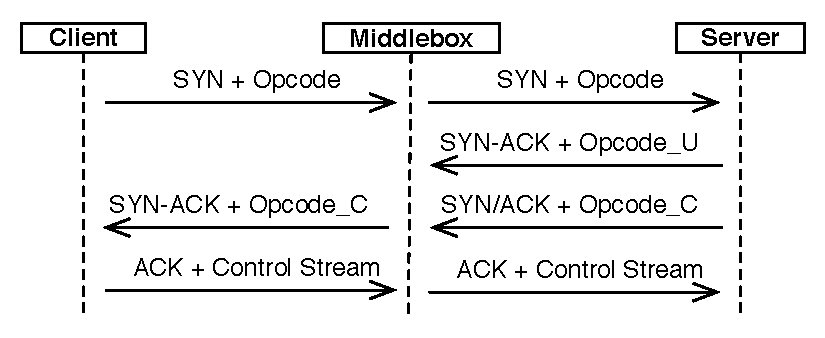
\includegraphics[width=.9\columnwidth]{figs/handshake}
% \vspace{-2mm}
\caption{Example handshake with extension negotiation}
\label{fig:handshake}
% \vspace{-4mm}
\end{figure}

Figure~\ref{fig:handshake} shows an example handshake. In this case a client sends a SYN packet as described above. The packet traverses a middlebox that does not remove the opcode and reaches the server. The server replies with SYN-ACK with $Opcode_U$, but the middlebox discards it. The server then retransmits SYN-ACK with $Opcode_C$ and Checksum Correction bits, delivered to the client. The client recovers and verifies the received opcode. Hence both endpoints understand the meaning of the opcode, therefore the client replies with an ACK with control information acknowledging $Opcode$ reception.

We witnessed one case of packet splitting where an ACK segment is split to one only acknowledging the received data and another other one with the actual payload. We did not observe a case where a middlebox both passes payload in SYN-ACK packet and splits ACK segments. If the handshake succeeds we need to take a little extra care with the fallback mechanism -- we need to wait for an ACK segment with payload before falling back to vanilla TCP. If the passive opener receives data it can not decode as valid TLV-encoded control information, it falls back to vanilla TCP.

Putting control stream information into packet payload suffers from much the same issues as other proposals to extend TCP option space~\cite{Ramaiah:2012wa}. The premise of our work is that middleboxes should not be aware of the new control streams in the first place and therefore not interfere with them. Currently we focus on exchanging control information within the packet header and leave refinement of the full control channel for future work.

\subsection{Control channel bitrate}

Our control channel does not need to protection from steganalysis as it is only used to avoid middlebox interference with end-to-end control information exchange. The bitrate of the channel without redefining part of packet payload for control information is bounded by the size of the TCP header (20 bytes without options), the round trip time (RTT) and the number of packets in flight per RTT. Depending on fields usable for a particular connection as inferred during the handshake, we can use between 16 (either $Opcode_C$ or $Opcode_U$) and 35 bits when using both fields and reserved flags.

For an operating window $cwnd$ (in bytes) a TCP flow has $cwnd/MSS$ data packets per RTT, hence that many headers can carry control data. If \emph{window scaling} option is not used, the maximum \emph{receive window} is 65536 bytes. Using the typical HSPA network RTT of about 100ms the maximum data rate is therefore 5 Mbit/s, reasonable for current networks~\cite{Chen:2012vj}. In this case covert channel bitrate is 7.0 to 15.4 kbit/s, depending on the fields used.

We can estimate channel bitrate from previously studies of 3G and 4G network characteristics~\cite{Chen:2012vj}. The average bandwidth measured for a large TCP transmission ranges from $1.2\pm 0.2$ Mbit/s for a 3G network and $348\pm 141$ ms RTT to $15.6\pm 1.0$ Mbit/s and $125\pm 41$ ms RTT for LTE. Covert channel bitrates for these cases range from $3.7 \pm 0.6$ kbit/s for 3G with one 16-bit field usable to $49.0 \pm 3.1$ kbit/s for LTE and both fields as well as reserved bits usable. Similarly, maximum bitrate of full-length option field is up to $34.5 \pm 5.7$ kbit/s and $448.2 \pm 28.7$ kbit/s for the two cases respectively.

Finally, the actual amount of information exchanged will depend on the coding scheme and the required reliability guarantees. For reliability in particular, a scheme described in Nusha~\cite{Rutkowska:2004ul} can be used.

For comparison, bitrates achievable by detection resistant schemes using initial sequence numbers are limited by only using the first packet in each connection to fit up to 15 bits of data~\cite{Murdoch:2005fz}. Using the same assumptions as before and establishing connections sequentially results in 150 bit/s when only SYN and SYN-ACK are exchanged, to 75 bit/s with complete handshake and teardown. 

\section{Related Work}
\label{sec:related}

Steganography has been used in the past to hide information within network protocols. The main focus has been on covert channels that violate system's security policy and initial sequence numbers~\cite{Rowland:1997vq}, TCP Timestamps~\cite{Giffin:2002wh} and combinations with IP flags~\cite{Murdoch:2005fz}. There are detection techniques for these methods, however our main goal is to exchange a small amount of control information rather than a genuine covert channel, calling for a different design.

TCP implements an \emph{urgent mechanism} that allows the sender to make the receiver accept some \emph{urgent data}. The mechanism is often quoted as providing ``out-of-bound'' data delivery and may be compelling to use for control information even though it is explicitly not designed as such. There are ambiguities regarding the semantics of the urgent pointer and Network Intrusion Detection Systems (NIDS) tend to clear the URG flag and pointer. Hence the general recommendation is not to use of the mechanism~\cite{Gont:2011vi}.

AccECN~\cite{Kuhlewind:2014vd} uses an additional reserved bit, overloads the meaning of already assigned ECN~\cite{Floyd:up} and NS~\cite{Ely:uc} bits and redefines Urgent Pointer as Non-Urgent when URG is not set. The idea is related to ours, but reserving the field solely for ECN use prevents other extensions from using it. Also, we saw that some networks block such packets, making it especially difficult to use for ECN.

Generic control stream for MPTCP~\cite{Bonaventure:wx} is another alternative. It proposes mapping the control stream into a separate sequence number space and exchanging control data over established subflows, only modifying the MPTCP DSS option to differentiate control and data streams. The underlying assumption, however, is that MPTCP is already deployed and that existing deployments will be compatible with the new specification.

\section{Discussion and Future Work}

The main points of discussion for \emph{NoTCP} are the same as with all TCP extensions: is it necessary, deployable and forwards-compatible? We have discussed the first two throughout the paper, but the biggest challenge for forwards-compatibility is NoTCP's overloading of header fields instead of using options. The exact protocol semantics are subject to further testing and discussions. The main goal of this work is to identify potential methods for exchanging control information by hiding it from existing middleboxes.

We have left open the question of finding a method to hide such information from non-transparent proxies. The easiest, albeit limited solution is to identify and cache port numbers that allow unmodified traffic. Instead we plan to study commonly found proxy implementations in detail in order to quickly identify them and encode information within their own operating patterns.

In the long term each protocol-related standard should explicitly define how it affects header fields. Examples include implicitly extending sequence number space~\cite{Mazieres:uz}, allowing encrypted TCP session to omit the timestamp option, using stronger message integrity checks making checksum field redundant, changing semantics of duplicate ACKs~\cite{Handley:vj,Flach:2013uy} or even simple window size modifications~\cite{Crowcroft:1998dk}.

We hope to map such header field modifications by existing extensions as well as network middlebox behavior patterns into an algebraic form as we have done in the simple case of checksum. Such definitions would allow us to go beyond the simple opcode exchange and signal detailed protocol information between endpoints using a low-bandwidth channel. Thus extending a protocol would become a matter of defining a new set of such header algebra rules hence simplifying the process of design and testing.

We have demonstrated the feasibility of using steganography to exchange end-to-end control information across current networks. Importantly, this is not a short term solution: TCP Fast Open is already being deployed and offers even more opportunities to hide information in the initial packets within higher-level protocol information, such as HTTP headers and cipher suites~\cite{Zielinska:2014fn}. Even if TCP was completely replaced by another protocol, opportunities for control information exchange remain.

\ifnum\anon=0
\subsection*{Acknowledgments}

\fi


\clearpage
%Only show things we really cite :)
% \nocite{*}
{

\bibliographystyle{abbrv}
\small 
\bibliography{references}
}

%\appendix 
%\input{data}

\end{document}







